\documentclass[journal]{IEEEtran}

\usepackage[utf8]{inputenc}
\usepackage[T1]{fontenc}
\usepackage{amsmath,amssymb,amsfonts}
\usepackage{graphicx}
\usepackage{booktabs}
\usepackage{array}
\usepackage{url}
\usepackage[hidelinks]{hyperref}
\usepackage{orcidlink}
\graphicspath{{../figures/}}

% IEEEtran hard-codes an em-dash after the abstract and index-terms names; the CAOS
% content standard (ADR-0067) excludes em-dashes, so the separator is a full stop.
\makeatletter
\def\abstract{\normalfont
    \if@twocolumn
      \@IEEEabskeysecsize\bfseries\textit{\abstractname}.\ \relax
    \else
      \bgroup\par\addvspace{0.5\baselineskip}\centering\vspace{-1.78ex}\@IEEEabskeysecsize\textbf{\abstractname}\par\addvspace{0.5\baselineskip}\egroup\quotation\@IEEEabskeysecsize
    \fi\@IEEEgobbleleadPARNLSP}
\def\IEEEkeywords{\normalfont
    \if@twocolumn
      \@IEEEabskeysecsize\bfseries\textit{\IEEEkeywordsname}.\ \relax
    \else
      \bgroup\par\addvspace{0.5\baselineskip}\centering\@IEEEabskeysecsize\textbf{\IEEEkeywordsname}\par\addvspace{0.5\baselineskip}\egroup\quotation\@IEEEabskeysecsize
    \fi\@IEEEgobbleleadPARNLSP}
\makeatother

% Page-1 header block (conventions/manuscript-header-standard.md). The four document
% macros are set by the publishing tool when the version DOI is reserved.
\newcommand{\doctype}{Preprint}
\newcommand{\docversion}{v2.3}
\newcommand{\docdate}{18 September 2026}
\newcommand{\versiondoi}{10.5281/zenodo.22825211}
\newcommand{\conceptdoi}{10.5281/zenodo.21509056}
\newcommand{\docrepo}{github.com/fsantibanezleal/CAOS\_RES\_Pulso}
\newcommand{\headerblock}{%
\begin{center}
\fbox{\parbox{0.94\textwidth}{\small\raggedright
\textbf{\doctype} \quad$\cdot$\quad \docversion, \docdate \quad$\cdot$\quad Licence CC BY 4.0\\[2pt]
CAOS open-research programme \quad$\cdot$\quad CAOS\_RES\_Pulso, cataloguing of pressure-transient flow behaviours\\[2pt]
Version DOI \href{https://doi.org/\versiondoi}{\texttt{\versiondoi}} \quad$\cdot$\quad
concept DOI (always latest) \href{https://doi.org/\conceptdoi}{\texttt{\conceptdoi}}\\[2pt]
Not peer reviewed. Source code, data and computational records: \href{https://\docrepo}{\texttt{\docrepo}}
}}
\end{center}}

\begin{document}

\title{Dual-Representation Mondrian Conformal Assignment of Pressure-Transient GeoTypes:
An Independent Reproduction and Extension for Fractured-Reservoir Flow}

\author{%
  Felipe Santib\'a\~nez-Leal~\orcidlink{0000-0002-0150-3246},~\IEEEmembership{Independent Researcher}%
  \thanks{F.\ Santib\'a\~nez-Leal is with the CAOS open-research programme, Santiago, Chile
    (e-mail: \texttt{fsantibanezleal@ug.uchile.cl}; ORCID: 0000-0002-0150-3246).}%
  \thanks{Code, derived artifacts, and the workbench are released under MIT at
    \url{https://github.com/fsantibanezleal/CAOS_RES_Pulso}; the reusable shape machinery is
    the Apache-2.0 package \texttt{pygeotypes}
    (\url{https://github.com/fsantibanezleal/CAOS_GeoTypes}). No GPL workflow code or raw
    licensed data is redistributed.}%
}

\markboth{\doctype\ \docversion, 2026 \textperiodcentered\ CAOS open-research programme}{Santib\'a\~nez-Leal:
Dual-Representation Mondrian Conformal Assignment of Pressure-Transient GeoTypes}

\IEEEaftertitletext{\vspace{-0.6\baselineskip}\headerblock\vspace{0.2\baselineskip}}

\IEEEtitleabstractindextext{%
\begin{abstract}
Fractured reservoirs exhibit recurring fluid-flow behaviours hidden in the shape of their
pressure-transient responses. A recent study clusters geologically consistent
discrete-fracture-network (DFN) ensembles into flow-behaviour classes and attributes each class
to fracture-network properties. We first independently reproduce that pipeline, DFN pressure
transients, Bourdet-derivative features, dynamic-time-warping (DTW) $k$-medoids clustering into a
GeoType catalogue, and random-forest / TreeSHAP attribution, from permissively licensed
components on the original open 4TU corpus and on analytic dual-porosity families. The
reproduction recovers clean clusters, with the real transients clustering more cleanly
(silhouette up to $0.86$) than the analytic families ($0.15$--$0.27$), and it recovers the
finding that fracture intensity ($\log I$) is a leading attributed control (top on two of the three
benchmark cases). We then extend the
pipeline in two ways. First, we make the assignment \emph{coverage-controlled}, which the base
random-forest attribution is not, with a class-conditional (Mondrian) split-conformal assigner on
a DTW nonconformity score that emits per-class $p$-values, a prediction set, and an
out-of-catalogue flag (empirical coverage $0.80$--$0.94$, straddling the $0.85$ target, across the rich-method cases).
Second, we apply a two-score (multi-view) \emph{dual-representation Mondrian
conformal} intersection that conformalizes jointly across two nonconformity scores, the DTW shape
distance and a physics-descriptor implausibility from the attribution forest, and accepts a
GeoType only in the per-class conjunction of the two prediction sets. This excludes curves that
are shape-close to the wrong physics, which single-score conformal accepts: across five
rich-method cases the dual conjunction trades marginal coverage (e.g.\ from $0.85$ to $0.73$ and from
$0.94$ to $0.87$) for tighter, physics-consistent sets. The shape machinery is signal-agnostic
and is exercised on real hydrogeology pumping-test field data as well as reservoir transients. The
contribution is a faithful, independent reproduction plus a coverage-controlled assignment that
fuses shape space and physics-descriptor space, with every number backed by a released
deterministic artifact.
\end{abstract}

\begin{IEEEkeywords}
fractured reservoirs, pressure-transient analysis, discrete fracture networks, dynamic time
warping, k-medoids, conformal prediction, Mondrian, random forests, SHAP, reproducibility,
geothermal, hydrogeology.
\end{IEEEkeywords}}

\maketitle
\IEEEdisplaynotcompsoctitleabstractindextext
\IEEEpeerreviewmaketitle

% =====================================================================
\section{Introduction}
% =====================================================================

\IEEEPARstart{T}{he} pressure-transient response of a well is a fingerprint of the reservoir's
flow structure: its shape, and the shape of its Bourdet derivative~\cite{bourdet1989},
distinguishes homogeneous from dual-porosity behaviour and localizes the interporosity
transition~\cite{warren1963}. In fractured reservoirs the mapping from geology to transient is
many-to-one and uncertain, so a natural question is whether the space of transients organizes into
a small catalogue of recurring flow behaviours, a ``geological DNA'', and if so, which
fracture-network properties control membership. A recent study answers both by clustering
geologically consistent discrete-fracture-network (DFN) ensembles into flow-behaviour classes and
attributing them~\cite{kameltarghi2026}.

This paper reproduces that pipeline and extends it with a coverage-controlled assignment.
Reproduction matters here for two reasons: the original workflow depends on a GPL-licensed code
base we deliberately do not vendor, and a clustering-plus-attribution result is only trustworthy
if an independent re-implementation on the same open data recovers it. We re-implement the shape
machinery from permissively licensed components, DTW~\cite{sakoe1978}, $k$-medoids, silhouette
selection~\cite{rousseeuw1987}, random forests~\cite{breiman2001}, and TreeSHAP~\cite{lundberg2020},
as the open package \texttt{pygeotypes}, run it on the original 4TU corpus~\cite{data4tu} and on
analytic dual-porosity families, and confirm the clusters and, on two of the three benchmark cases,
the top attributed control. The
extension addresses a gap in how such catalogues are \emph{used}: random-forest attribution ranks
controls but gives no guarantee on a new curve's class, and a curve can be shape-close to the wrong
physics. We therefore add conformal prediction~\cite{vovk2005,angelopoulos2023}, first a
class-conditional (Mondrian) split-conformal assigner on the shape distance, then a
dual-representation variant that conformalizes jointly over shape and physics-descriptor scores.
Our contributions are: (i) an independent, permissively licensed reproduction of the DFN-transient
GeoType pipeline that recovers its clusters and partially recovers its fracture-intensity
attribution; (ii) a
coverage-controlled Mondrian conformal GeoType assigner; (iii) a dual-representation Mondrian
conformal assigner that excludes right-shape-wrong-physics curves, with its coverage/tightness
trade-off quantified.

% =====================================================================
\section{Reproduced pipeline}
\label{sec:pipeline}
% =====================================================================

A GeoType catalogue is built in four stages. \emph{Transients and features.} Each DFN ensemble (or
analytic study) yields pressure transients; from each we compute the log-time pressure and its
Bourdet derivative~\cite{bourdet1989}, and for analytic dual-porosity references the Warren--Root
response~\cite{warren1963} is evaluated by Stehfest numerical Laplace inversion~\cite{stehfest1970}.
\emph{Clustering.} Curves are compared by dynamic time warping~\cite{sakoe1978} and grouped by
$k$-medoids; the catalogue size $K$ is chosen by a silhouette sweep~\cite{rousseeuw1987}, and each
GeoType is represented by its medoid curve and a membership (Fig.~\ref{fig:catalogue}).
\emph{Attribution.} A random forest~\cite{breiman2001} predicts the GeoType from physical
descriptors, subject to an accuracy threshold (attribution is withheld when the forest cannot
predict the labels), and TreeSHAP~\cite{lundberg2020} ranks the controlling descriptors.
\emph{Assignment.} A new curve is classified against the precomputed medoids.

\begin{figure}[!t]
\centering
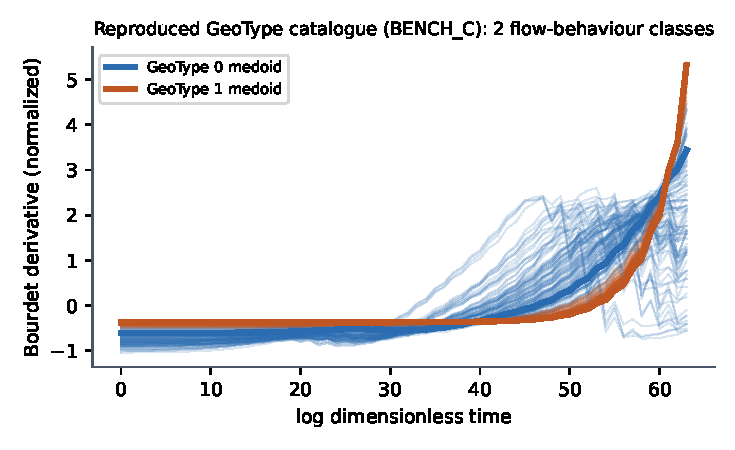
\includegraphics[width=\columnwidth]{fig-catalogue.pdf}
\caption{A reproduced GeoType catalogue (case BENCH\_C): the member Bourdet-derivative curves
coloured by GeoType, with the two medoids in bold. Data: \texttt{trace.json}.}
\label{fig:catalogue}
\end{figure}

\begin{figure}[!t]
\centering
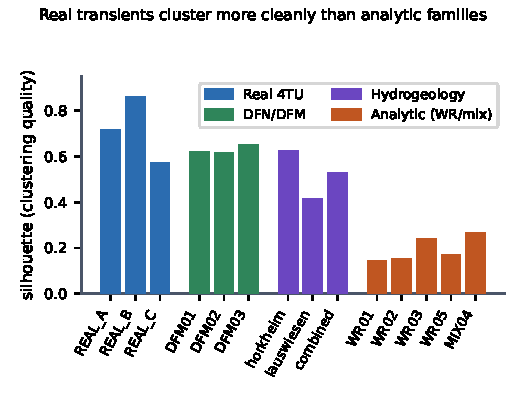
\includegraphics[width=\columnwidth]{fig-silhouette.pdf}
\caption{Clustering quality (silhouette) per case, grouped by family. The real 4TU transients
cluster more cleanly (up to $0.86$) than the analytic Warren--Root families ($0.15$--$0.27$), with
the DFN/DFM and hydrogeology cases in between. Data: the per-case \texttt{trace.json} files.}
\label{fig:silhouette}
\end{figure}

On the original open corpus the reproduction recovers the reported structure
(Fig.~\ref{fig:silhouette}): the real 4TU transients cluster more cleanly than the analytic
families. Fracture intensity ($\log I$, absorbing its $\rho\!>\!0.9$ correlates) is the top
attributed control (largest mean absolute SHAP) on two of the three 4TU-benchmark cases (BENCH\_A,
BENCH\_C) and second on BENCH\_B, where the fraction of fractures in the largest connected component
leads; on the real-4TU cases other descriptors lead (aperture, the fracture-length exponent, and
permeability, with $\log I$ a close second on REAL\_C), and on the Warren--Root families $\lambda$
leads. This partially reproduces the paper's fracture-intensity finding.
On the analytic families the interporosity flow coefficient $\log_{10}\lambda$ dominates the
assignment sensitivity, exactly as the physics predicts, since $\lambda$ sets the transition timing
that separates the dual-porosity behaviours. The same permissively licensed pipeline, exercised over
twenty-one cases (analytic Warren--Root and mixture studies, real 4TU datasets, DFN/DFM
network ensembles, and hydrogeology field sites; Appendix~\ref{ap:cases}), is a complete method
ladder: classical pressure-transient analysis, DTW $k$-medoids clustering, silhouette-selected
catalogue size, random-forest / TreeSHAP attribution, and the conformal assignment below.

% =====================================================================
\section{Coverage-controlled assignment}
\label{sec:conformal}
% =====================================================================

\subsection{Mondrian split-conformal on the shape score}

Random-forest attribution ranks controls but offers no guarantee that a new curve is assigned to
the right GeoType. We add a class-conditional (Mondrian) split-conformal
assigner~\cite{vovk2005,angelopoulos2023}. The nonconformity score of a curve $x$ for GeoType $g$
is its DTW distance to the medoid, $s_\text{shape}(x,g)$. Calibrated per class on a disjoint slice,
it yields a $p$-value $p_\text{shape}(x,g)$ and a prediction set
$\{g:p_\text{shape}(x,g)>\alpha\}$; a curve matching no class is flagged out-of-catalogue. Across
the rich-method cases the empirical marginal coverage is $0.80$--$0.94$, straddling the target level, with an
out-of-catalogue rate of $0.03$--$0.17$: a coverage guarantee the base attribution cannot give.

\subsection{Dual-representation Mondrian conformal assignment}

A single score cannot express that a curve may be shape-close to the wrong physics: a transient
that matches a medoid by DTW shape yet whose physical descriptors are atypical for that GeoType. We
conformalize jointly across two representations. In addition to the shape score, define a descriptor
score
\begin{equation}
s_\text{desc}(x,g)=1-\mathrm{RF}\big(g\mid\text{descriptors}(x)\big),
\end{equation}
the implausibility of $x$'s physical descriptors under GeoType $g$ from the attribution forest.
Both are Mondrian-calibrated, giving $p_\text{shape}$ and $p_\text{desc}$, and the dual prediction
set is the per-class conjunction
\begin{equation}
\Gamma^\alpha(x)=\big\{\,g:p_\text{shape}(x,g)>\alpha\ \wedge\ p_\text{desc}(x,g)>\alpha\,\big\}.
\label{eq:dual}
\end{equation}
A GeoType is accepted only if the curve is both shape-consistent and descriptor-consistent; a shape
match with implausible physics is excluded. Intersecting independently calibrated conformal sets
across representations is an established multi-view/multi-score construction~\cite{garciaceja2024mv,xu2025alpha};
our contribution is its \emph{application}, fusing a DTW shape score with a random-forest
descriptor-implausibility score for pressure-transient GeoType assignment, and the measured
coverage/tightness trade-off. Because the per-class conjunction is a Bonferroni-style combination, its
marginal coverage is only guaranteed at $1-2\alpha$. In practice it falls below the target
$1-\alpha=0.85$ in four of the five rich-method cases (WR01, BENCH\_A, BENCH\_B, BENCH\_C) but not
on REAL\_A ($0.87$), and below the shape-only coverage in all five, which is precisely the coverage
cost we report.

Fig.~\ref{fig:dual} shows the trade-off across five rich-method cases. The dual conjunction
tightens the mean set size and flags right-shape-wrong-physics curves that shape-only conformal
accepts, at the cost of some marginal coverage (for example from $0.85$ to $0.73$ on BENCH\_A and
from $0.94$ to $0.87$ on REAL\_A). When descriptors are absent or degenerate (some real cases), the dual
layer degrades gracefully to shape-only and reports that it did.

\begin{figure}[!t]
\centering
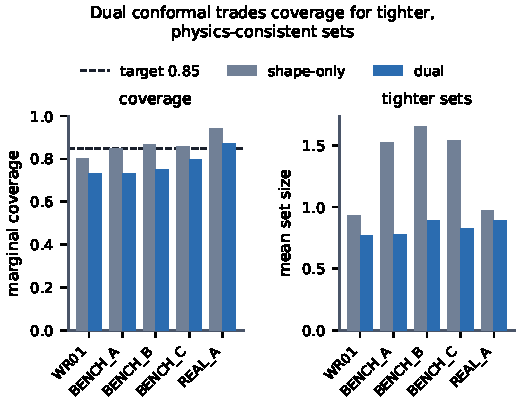
\includegraphics[width=\columnwidth]{fig-dual-conformal.pdf}
\caption{Dual-representation vs shape-only Mondrian conformal across five rich-method cases. The
dual conjunction trades marginal coverage (left) for tighter, physics-consistent prediction sets
(right), excluding curves that are shape-close to the wrong physics. The dashed line marks the
target coverage $1-\alpha=0.85$. Data: the \texttt{attribution\_plus.dual\_conformal} block of each
\texttt{trace.json}.}
\label{fig:dual}
\end{figure}

% =====================================================================
\section{Generalization and scope}
% =====================================================================

The shape machinery is signal-agnostic: any response signal whose shape reflects the underlying
physical system, hydrogeology pumping tests, geothermal and thermal-response tests, can be
catalogued and conformally assigned by the same code. We exercise it on real hydrogeology
pumping-test field data (the Horkheim and Lauswiesen sites) alongside the reservoir transients, all
through one pipeline (Appendix~\ref{ap:cases}).

This is a reproduction plus extension of a published pipeline, not a wholly new method for the base
clustering and attribution, which are credited to the reproduced work. The DFN pressure-transient
simulation on the full open-source flow engine is an offline dependency that is not integrated end
to end; the results here rest on the reproduced study's published corpus, analytic dual-porosity
families, DFN ensembles, and field data, and the artifacts that lack a simulated transient carry an
explicit pending flag rather than a fabricated curve. The dual-conformal coverage is a trade-off: it
buys physics-consistency and tighter sets at the price of marginal coverage, and both sides are
shown. Every number comes from a released, seed-deterministic artifact.

% =====================================================================
\section{Conclusion}
% =====================================================================

We independently reproduced, from permissively licensed components, a DFN-transient GeoType pipeline
for fractured-reservoir flow, recovering its clusters (silhouette up to $0.86$, real transients
cleaner than analytic) and, partially, its fracture-intensity attribution (fracture intensity is the
top attributed control on two of the three benchmark cases), and extended it with a
coverage-controlled Mondrian conformal assigner and, as the methodological contribution, a
dual-representation Mondrian conformal assigner that fuses shape and physics-descriptor evidence to
exclude right-shape-wrong-physics assignments. The result is a reproducible, coverage-controlled way
to place a new pressure transient in a catalogue of flow behaviours and to say, with a guarantee,
when it belongs to none.

% =====================================================================
\section*{Data and code availability}
% =====================================================================

{\raggedright
Code, the derived artifacts, and the workbench are at
\url{https://github.com/fsantibanezleal/CAOS_RES_Pulso} (MIT); the reusable shape machinery is
\texttt{pygeotypes} (Apache-2.0). The reference corpus is the open 4TU dataset of the reproduced
study~\cite{data4tu} (GPL-3.0; used locally and not redistributed); GPL workflow code is not
included. Only compact derived artifacts are distributed. The figures are regenerated
deterministically from these traces by
\path{manuscripts/dual-conformal-geotypes/figures/make_figs.py}.\par}

\appendices
\section{Per-case results}
\label{ap:cases}
The pipeline was run over twenty-one cases. Representative silhouette, out-of-catalogue
rate, and (where the dual layer runs) the shape-only and dual coverage are: REAL\_A $0.72$ /
shape-only $0.94$, dual $0.87$; REAL\_B $0.86$; REAL\_C $0.58$; BENCH\_A $0.57$ / shape-only $0.85$, dual $0.73$;
BENCH\_B $0.48$ / shape-only $0.87$, dual $0.75$; BENCH\_C $0.62$ / shape-only $0.86$, dual $0.80$; DFM01 $0.62$; DFM03 $0.65$;
FIELD\_horkheim $0.62$; FIELD\_lauswiesen $0.42$; WR01 $0.15$ / shape-only $0.80$, dual $0.73$; the analytic WR
and mixture families $0.15$--$0.27$. The full per-case table (silhouette, $K$, coverage,
out-of-catalogue rate, mean set size, dual comparison, and attribution) is stored in each case's
\texttt{trace.json}.

% =====================================================================
\begin{thebibliography}{99}
\itemsep 1pt

\bibitem{kameltarghi2026} E.~Kamel Targhi, G.~Rongier, P.-O. Bruna, A.~Daniilidis, and S.~Geiger,
``Unsupervised learning for geologically consistent fluid flow analysis in fractured reservoirs,''
\emph{Comput. Geosci.}, vol.~30, 57, 2026, doi:10.1007/s10596-026-10459-w.
\bibitem{warren1963} J.~E. Warren and P.~J. Root, ``The behavior of naturally fractured reservoirs,''
\emph{SPE J.}, vol.~3, no.~3, pp.~245--255, 1963, doi:10.2118/426-PA.
\bibitem{bourdet1989} D.~Bourdet, J.~A. Ayoub, and Y.~M. Pirard, ``Use of pressure derivative in
well-test interpretation,'' \emph{SPE Formation Eval.}, vol.~4, no.~2, pp.~293--302, 1989,
doi:10.2118/12777-PA.
\bibitem{stehfest1970} H.~Stehfest, ``Algorithm 368: Numerical inversion of Laplace transforms,''
\emph{Commun. ACM}, vol.~13, no.~1, pp.~47--49, 1970, doi:10.1145/361953.361969.
\bibitem{sakoe1978} H.~Sakoe and S.~Chiba, ``Dynamic programming algorithm optimization for spoken
word recognition,'' \emph{IEEE Trans. Acoust., Speech, Signal Process.}, vol.~26, no.~1,
pp.~43--49, 1978, doi:10.1109/TASSP.1978.1163055.
\bibitem{rousseeuw1987} P.~J. Rousseeuw, ``Silhouettes: A graphical aid to the interpretation and
validation of cluster analysis,'' \emph{J. Comput. Appl. Math.}, vol.~20, pp.~53--65, 1987,
doi:10.1016/0377-0427(87)90125-7.
\bibitem{breiman2001} L.~Breiman, ``Random forests,'' \emph{Mach. Learn.}, vol.~45, no.~1,
pp.~5--32, 2001, doi:10.1023/A:1010933404324.
\bibitem{lundberg2020} S.~M. Lundberg \emph{et al.}, ``From local explanations to global
understanding with explainable AI for trees,'' \emph{Nat. Mach. Intell.}, vol.~2, pp.~56--67,
2020, doi:10.1038/s42256-019-0138-9.
\bibitem{vovk2005} V.~Vovk, A.~Gammerman, and G.~Shafer, \emph{Algorithmic Learning in a Random
World}. New York: Springer, 2005, doi:10.1007/b106715.
\bibitem{angelopoulos2023} A.~N. Angelopoulos and S.~Bates, ``Conformal prediction: A gentle
introduction,'' \emph{Found. Trends Mach. Learn.}, vol.~16, no.~4, pp.~494--591, 2023,
doi:10.1561/2200000101.
\bibitem{garciaceja2024mv} E.~Garcia-Ceja, ``Multi-view conformal learning for heterogeneous
sensor fusion,'' 2024. arXiv:2402.12307.
\bibitem{xu2025alpha} C.~Xu, Y.~Yu, and H.~Ren, ``Aggregating conformal prediction sets via
$\alpha$-allocation,'' 2025. arXiv:2511.12065.
\bibitem{data4tu} E.~Kamel Targhi \emph{et al.}, ``Data and code supporting: Unsupervised learning
workflow for clustering pressure transient responses in fractured reservoirs (dataset),''
4TU.ResearchData, 2026,
doi:10.4121/8291d285-025d-4724-988d-fc747a578c0a.

\end{thebibliography}

\end{document}
